%%%%%%%%%%%%%%%%%%%%%%%%%%%%%%%%%%%%%%%%%%%%%%%%%%%%%%%%%%%%%%%%%%%%%%%%%%%%%%%
\section{Data flow dependency}
%%%%%%%%%%%%%%%%%%%%%%%%%%%%%%%%%%%%%%%%%%%%%%%%%%%%%%%%%%%%%%%%%%%%%%%%%%%%%%%
%------------------------------------------------------------------------------
%%%%%%%%%%%%%%%%%%%%%%%%%%%%%%%%%%%%%%%%%%%%%%%%%%%%%%%%%%%%%%%%%%%%%%%%%%%%%%%
\subsection{Data flow dependency}
%------------------------------------------------------------------------------
\begin{frame}
  \frametitle{Data flow dependency}
  \begin{block}{Concept}
    Similar to a DAG of tasks, but combines {\bf task dependencies with data-driven execution}.
    \begin{itemize}
    \item Execution is controlled by the {\bf Data Flow Graph (DFG)}.
    \item Unlike the program recursion structure of {\bf full strict model}.
    \end{itemize}
  \end{block}
  %
  \vspace{-4mm}
  %
  \begin{columns}
    \begin{column}{0.5\textwidth}
      \begin{center}
	{\bf Fully strict mode (Cilk)}
      \end{center}
    \end{column}
    %
    \begin{column}{0.5\textwidth}
      \begin{center}
	{\bf Data flow graph}
      \end{center}
    \end{column}
  \end{columns}
  %
  \vspace{-2mm}
  %
  \begin{columns}
    \begin{column}{0.5\textwidth}
      \begin{center}
	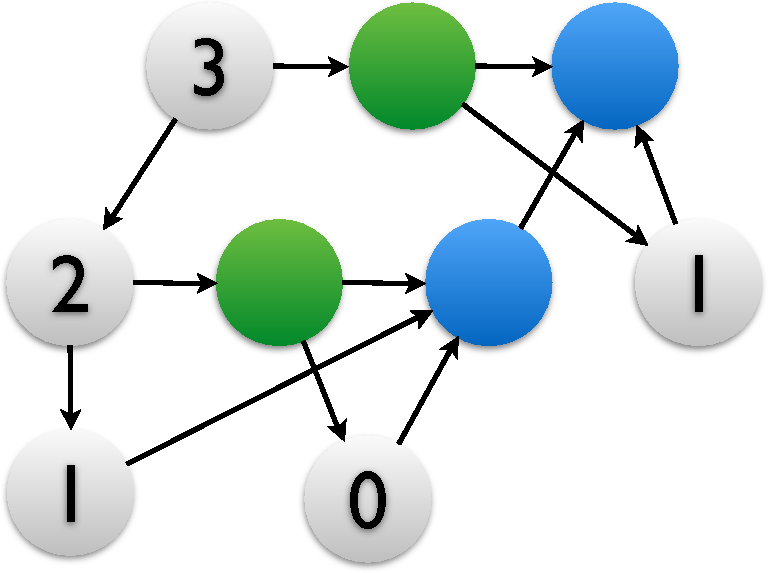
\includegraphics[width=0.8\textwidth]{dag-strict-crop}
      \end{center}
    \end{column}
    %
    \begin{column}{0.5\textwidth}
      \begin{center}
	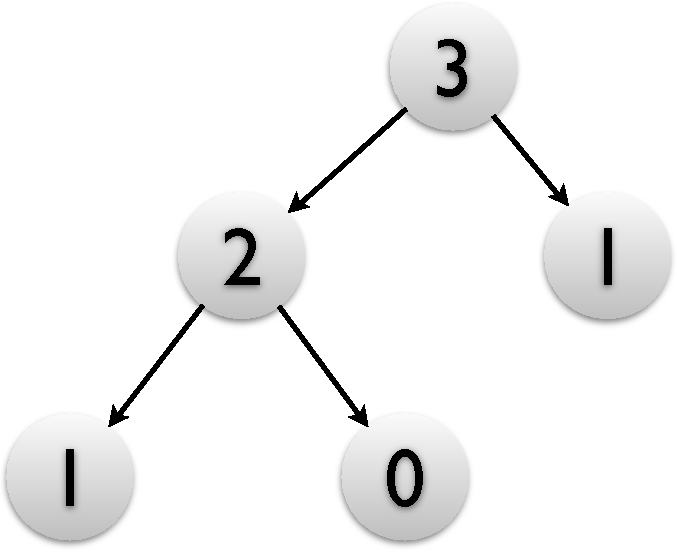
\includegraphics[width=0.8\textwidth]{dag-dfg-crop}
      \end{center}
    \end{column}
  \end{columns}
\end{frame}
%------------------------------------------------------------------------------
\begin{frame}
  \frametitle{Data flow dependency}
  \begin{exampleblock}{Data access modes}
    \begin{itemize}[<+->]
    \item \blue{Read only}  ({\bf RO or R}) - only read, no permission to modify.
    \item \blue{Write only}  ({\bf WO or W}) - only write, no wait for data inputs.
    \item \blue{Read and Write} ({\bf RW}) - or exclusive mode, read and write.
    \item \blue{Cumulative Write} ({\bf CW}) - concurrent write and cumulative.
    \end{itemize}
  \end{exampleblock}
\end{frame}
%------------------------------------------------------------------------------
\begin{frame}[fragile]
  \frametitle{Data flow dependency}
  The concepts here \red{are the same} from \blue{computer architecture} in which
  we can replace {\bf instruction} by {\bf task}.
  %
  \begin{block}{Data dependencies}
    \begin{itemize}
    \item Task $t_i$ produces a result that may be used by a task $t_j$.
    \item Task $t_j$ is data dependent on task $t_k$, and $t_k$ is 
    data dependent on $t_i$ ($t_i \rightarrow t_k \rightarrow t_j$). 
    \end{itemize}
  \end{block}
  %
  \vspace*{-4mm}
  %
  \begin{columns}
  \begin{column}{0.6\textwidth}
  \begin{flushright}
  \begin{block}{}
\begin{lstlisting}
compute( input, &result );

display( &result );
\end{lstlisting}
  \end{block}
  \end{flushright}
  \end{column}
  %
    \begin{column}{0.4\textwidth}
      \begin{flushleft}
	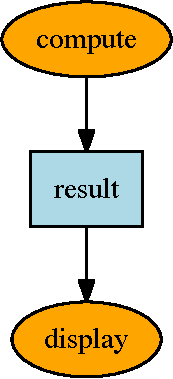
\includegraphics[width=0.4\textwidth]{dependency-crop}
      \end{flushleft}
    \end{column}
  \end{columns}
  %
\begin{tikzpicture}[overlay,>=stealth]
\draw<2-> [->,line width=2pt,red] (2.9, 2.6) .. controls(2.4, 2.2) .. (1.9, 2) node {};
\end{tikzpicture}
\end{frame}
%------------------------------------------------------------------------------
%\begin{frame}
%  \frametitle{Flow dependency}
%  \begin{exampleblock}{Flow dependency}
%    Ou dependência de dados, \emph{data dependency}, \emph{true dependency}, ou 
%    \textbf{read-after-write (RAW)} onde uma tarefa depende do resultado produzido
%    por uma tarefa anterior.
%  \end{exampleblock}
%  \begin{center}
%    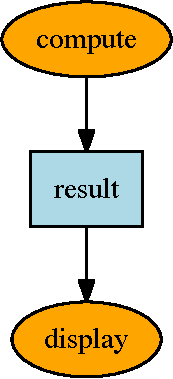
\includegraphics[scale=0.6]{dependency-crop}
%  \end{center}
%\end{frame}
%------------------------------------------------------------------------------
\begin{frame}
  \frametitle{Data hazards}
  \begin{alertblock}{Data hazards}
  There is a \textbf{dependence} between task and the we must preserve the execution order. 
  %
    \begin{itemize}
    \item \textbf{RAW} (\emph{Read after Write}).
    \item \textbf{WAW} (\emph{Write after Write}).
    \item \textbf{WAR} (\emph{Write after Read}).
    \end{itemize}
  \end{alertblock}
  %
\end{frame}
%------------------------------------------------------------------------------
%------------------------------------------------------------------------------
%------------------------------------------------------------------------------
\begin{frame}
  \frametitle{Data flow dependency}
%  \vspace*{-4cm}
  \begin{columns}
  \begin{column}{0.4\textwidth}
	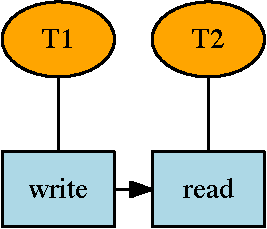
\includegraphics[width=\textwidth]{read-after-write-crop}
  \end{column}
  %
  \begin{column}{0.6\textwidth}
    \begin{itemize}
    \item \textbf{RAW} (\emph{Read after Write}) - or \blue{true dependency}, \blue{data dependency}.
    \item A task depends on the result produced by a previous task.
    \end{itemize}
  \end{column}
  \end{columns}
\end{frame}
%------------------------------------------------------------------------------
\begin{frame}
  \frametitle{Data flow dependency}
  \begin{columns}
  \begin{column}{0.4\textwidth}
	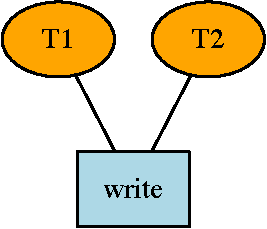
\includegraphics[width=\textwidth]{write-after-write-crop}
  \end{column}
  %
  \begin{column}{0.6\textwidth}
    \begin{itemize}
    \item \textbf{WAW} (\emph{Write after Write}) - or \blue{output dependency}.
    \item The execution order will affect the final output.
    \end{itemize}
  \end{column}
  \end{columns}
\end{frame}
%------------------------------------------------------------------------------
\begin{frame}
  \frametitle{Data flow dependency}
  \begin{columns}
  \begin{column}{0.4\textwidth}
	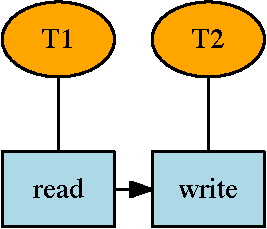
\includegraphics[width=\textwidth]{write-after-read-crop}
  \end{column}
  %
  \begin{column}{0.6\textwidth}
    \begin{itemize}
    \item \textbf{WAR} (\emph{Write after Read}) - or \blue{anti-dependency}.
    \item A task writes a value before it is read.
    \end{itemize}
  \end{column}
  \end{columns}
\end{frame}
%------------------------------------------------------------------------------
%%%%%%%%%%%%%%%%%%%%%%%%%%%%%%%%%%%%%%%%%%%%%%%%%%%%%%%%%%%%%%%%%%%%%%%%%%%%%%%
\subsection{Data flow example}
%------------------------------------------------------------------------------
\begin{frame}[fragile]
  \frametitle{Data flow example}
  In our next examples, we will use the following keywords:
  \begin{itemize}
  \item \textbf{in} - read access.
  \item \textbf{out} - write access.
  \item \textbf{inout} - read and write access.
  \end{itemize}
  %
\begin{block}{}
\begin{lstlisting}
void reading(in int a) {}
void modifying(inout int b) {}
main(void)
{
  int a;
  reading( a );
  reading( a );
  reading( a );
  modifying( a );
  modifying( a );
}
\end{lstlisting}
\end{block}
%  \begin{code}\footnotesize
%void reading(in int a)
%\{
%  \emph{\color{OliveGreen}{/* code here */}}
%\}
%void modifying(inout int b)
%\{
%  \emph{\color{OliveGreen}{/* code here to modify data */}}
%\}
%main(void)
%\{
%  int a;
%  reading( a );
%  reading( a );
%  reading( a );
%  modifying( a );
%  modifying( a );
%\}
%  \end{code}
\end{frame}
%------------------------------------------------------------------------------
\begin{frame}[fragile]
  \frametitle{Data flow example}
  \begin{columns}
  \begin{column}{0.6\textwidth}
\begin{block}{}
\begin{lstlisting}[escapeinside={@}{@}]
void reading(in int a) {}
void modifying(inout int b) {}
main(void)
{
  int a;
  @\alert<2>{reading( a );}@
  @\alert<3>{reading( a );}@
  @\alert<4>{reading( a );}@
  @\alert<5>{modifying( a );}@
  @\alert<6>{modifying( a );}@
}
\end{lstlisting}
%  @{\bfseries\color{Red}{modifying( a );}}@
\end{block}
  \end{column}
  \begin{column}{0.4\textwidth}
  \hspace{10mm}
  \begin{tikzpicture}[node distance=1.5cm,overlay,>=stealth]
  \tikzstyle{task}=[shape=circle,draw,thick,inner sep=0pt,minimum size=25pt,draw=black,fill=blue!20]
  \tikzstyle{mode}=[shape=rectangle,draw,thick,inner sep=0pt,minimum size=30pt,draw=black,fill=red!20]
  \node<2-> [task] (t1) {{\large$t_1$}};
  \node<2-> [task] (t2) [below of=t1] {{\large$t_2$}};
  \node<2-> [task] (t3) [below of=t2] {{\large$t_3$}};
  \node<2-> [mode] (m1) [right of=t2] {{\large\bf R}};
  \path<2-> (m1) edge [thick] (t1);
  \path<3-> (m1) edge [thick] (t2);
  \path<4-> (m1) edge [thick] (t3);
  %
  \node<5-> [task] (t4) [below of=t3] {{\large$t_4$}};
  \node<5-> [mode] (m2) [right of=t4] {{\large\bf RW}};
  \path<5-> (m2) edge [thick] (t4);
  \path<5-> (m2) edge [<-,thick] (m1);
  %
  \node<6-> [task] (t5) [below of=t4] {{\large$t_5$}};
  \node<6-> [mode] (m3) [right of=t5] {{\large\bf RW}}
    edge [thick] (t5)
    edge [<-,thick] (m2);
  \end{tikzpicture}
  \vspace{60mm}
  \end{column}
  \end{columns}
\end{frame}
%------------------------------------------------------------------------------
%------------------------------------------------------------------------------
%------------------------------------------------------------------------------
\begin{frame}[fragile]
  \frametitle{Fibonacci example}
\begin{block}{}
\begin{lstlisting}
void fibo( int n, int* res )
{
  int x, y;
  if( n < 2 ){
    *res = n;
  } else {
    fibo( n-1, &x );
    fibo( n-2, &y );
    *res = x+y;
  }
}

int main(void) {
  int n = 3, res;
  fibo( n, &res );
  print( res );
  return 0;
}
\end{lstlisting}
\end{block}
\end{frame}
%------------------------------------------------------------------------------
\begin{frame}[fragile]
  \frametitle{Fibonacci example}
  \begin{alertblock}{Notice}
    This recursive Fibonacci is not the best implementation, but it serves our purposes.
  \end{alertblock}
  %
  \pause
  %
  \begin{exampleblock}{Dependency example (again)}
    In our next example, we will use the following keywords:
    \begin{itemize}
    \item \textbf{in} - read access.
    \item \textbf{out} - write access.
    \item \textbf{inout} - read and write access.
    \item \textbf{cout} - cumulative write with global reduction.
    \end{itemize}
  \end{exampleblock}
\end{frame}
%------------------------------------------------------------------------------
\begin{frame}[fragile]
  \frametitle{Fibonacci example}
\begin{block}{}
\begin{lstlisting}
void fibo( in int n, out int* res )
{
  int x, y;
  if( n < 2 ){
    *res = n;
  } else {
    fibo( n-1, &x );
    fibo( n-2, &y );
    *res = x+y;
  }
}

int main(void) {
  int n = 3, res;
  fibo( n, &res );
  print( res );
  return 0;
}
\end{lstlisting}
\end{block}
%
\begin{tikzpicture}[overlay,>=stealth]
\draw<2-> [draw=red,very thick] (1.4,3.8) ellipse (30pt and 10pt);
\end{tikzpicture}
%
\end{frame}
%------------------------------------------------------------------------------
\begin{frame}[fragile]
  \frametitle{Fibonacci example}
\begin{block}{Previous Fibonacci example}
\begin{lstlisting}[firstnumber=6]
  } else {
    fibo( n-1, &x );
    fibo( n-2, &y );
    *res = x+y;
  }
\end{lstlisting}
\end{block}
%
\pause
%
\begin{alertblock}{Synchronization problem}
If our tasks execute in parallel, we would like \textbf{to wait} for the
results from the previous two \texttt{fibo} tasks.
\end{alertblock}
%
\pause
%
\begin{exampleblock}{Solution}
  \begin{enumerate}
  \item An explicit synchronization (Cilk's style).
  \item A task that depends on the results from the two \texttt{fibo} tasks.
  \end{enumerate}
\end{exampleblock}
%
\end{frame}
%------------------------------------------------------------------------------
\begin{frame}[fragile]
  \frametitle{Fibonacci example}
\begin{block}{}
\begin{lstlisting}
void sum( out int* res, in int x, in int y )
{
  *a = x + y;
}

void fibo( in int n, out int* res )
{
  int x, y;
  if( n < 2 ){
    *res = n;
  } else {
    fibo( n-1, &x );
    fibo( n-2, &y );
    sum( res, x, y );
  }
}
\end{lstlisting}
\end{block}
%
\begin{tikzpicture}[overlay,>=stealth]
\draw<2-> [draw=red,very thick] (1.8,1.5) ellipse (40pt and 10pt);
\end{tikzpicture}
%
\end{frame}
%------------------------------------------------------------------------------
\begin{frame}[fragile]
  \frametitle{Fibonacci example (cumulative)}
\begin{block}{}
\begin{lstlisting}
void fibo( in int n, cout int* res )
{
  int x, y;
  if( n < 2 ){
    *res += n;
  } else {
    fibo( n-1, &x );
    fibo( n-2, &y );
  }
}
\end{lstlisting}
\end{block}
%
\begin{tikzpicture}[overlay,>=stealth]
\draw<2-> [draw=red,very thick] (1.5,2.5) ellipse (30pt and 10pt);
\draw<2-> [draw=red,very thick] (3.8,3.9) ellipse (15pt and 10pt);
\end{tikzpicture}
%
\end{frame}
%------------------------------------------------------------------------------
%\begin{frame}
%  \frametitle{Data flow dependency}
%  \vspace*{-4cm}
%  \begin{tikzpicture}[node distance=1.5cm,overlay,>=stealth]
%  \tikzstyle{task}=[shape=circle,draw,thick,inner sep=0pt,minimum size=25pt,draw=black,fill=blue!20]
%  \tikzstyle{mode}=[shape=rectangle,draw,thick,inner sep=0pt,minimum size=30pt,draw=black,fill=red!20]
%%  \path[use as bounding box] (-1,0) rectangle(10,-2);
%  \node[task] (t1) {{\large$t_1$}};
%  \node[mode] (m1) [below of=t1] {{\large\bf RW}}
%    edge [thick] (t1);
%  %
%  \node[task] (t2) [right of=t1] {{\large$t_2$}};
%  \node[task] (t3) [right of=t2] {{\large$t_3$}};
%  \node[mode] (m2) [below of=t2] {{\large\bf R}}
%    edge [thick] (t2)
%    edge [thick] (t3)
%    edge [<-,thick] (m1);
%  %
%  \node[task] (t4) [right of=t3] {{\large$t_4$}};
%  \node[mode] (m3) [below of=t4] {{\large\bf W}}
%    edge [thick] (t4)
%    edge [<-,thick] (m2);
%  %
%  \node[task] (t5) [right of=t4] {{\large$t_5$}};
%  \node[task] (t6) [right of=t5] {{\large$t_6$}};
%  \node[task] (t7) [right of=t6] {{\large$t_7$}};
%  \node[mode] (m4) [below of=t6] {{\large\bf CW}}
%    edge [thick] (t5)
%    edge [thick] (t6)
%    edge [thick] (t7)
%    edge [<-,thick] (m3);
%  \node[task] (taa) [below of=m1] {{\large$t_i$}};
%  \node (ttaa) [right of=taa,right] {{\large Nó tarefa}};
%  \node[mode] (maa) [below of=taa] {{\large R}};
%  \node  [right of=maa,right] {{\large Nó de modo de acesso}};
%  \end{tikzpicture}
%\end{frame}
%------------------------------------------------------------------------------
%%%%%%%%%%%%%%%%%%%%%%%%%%%%%%%%%%%%%%%%%%%%%%%%%%%%%%%%%%%%%%%%%%%%%%%%%%%%%%%
\subsection{Data flow graph}
%------------------------------------------------------------------------------
\begin{frame}
  \frametitle{Data flow graph}
  \begin{itemize}
  \item Data flow graph (DFG) combines task dependencies with data driven execution.
  \end{itemize}
  %
  \vspace{-4mm}
  %
  \begin{columns}
    \begin{column}{0.5\textwidth}
      \begin{center}
	{\bf Fully strict mode (Cilk)}
      \end{center}
    \end{column}
    %
    \begin{column}{0.5\textwidth}
      \begin{center}
	{\bf Data flow graph}
      \end{center}
    \end{column}
  \end{columns}
  %
  \vspace{-2mm}
  %
  \begin{columns}
    \begin{column}{0.5\textwidth}
      \begin{center}
	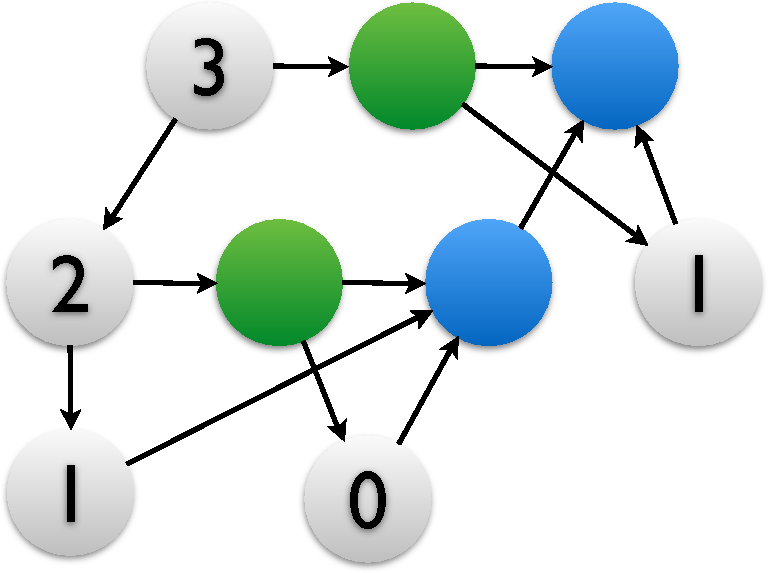
\includegraphics[width=\textwidth]{dag-strict-crop}
      \end{center}
    \end{column}
    %
    \begin{column}{0.5\textwidth}
      \begin{center}
	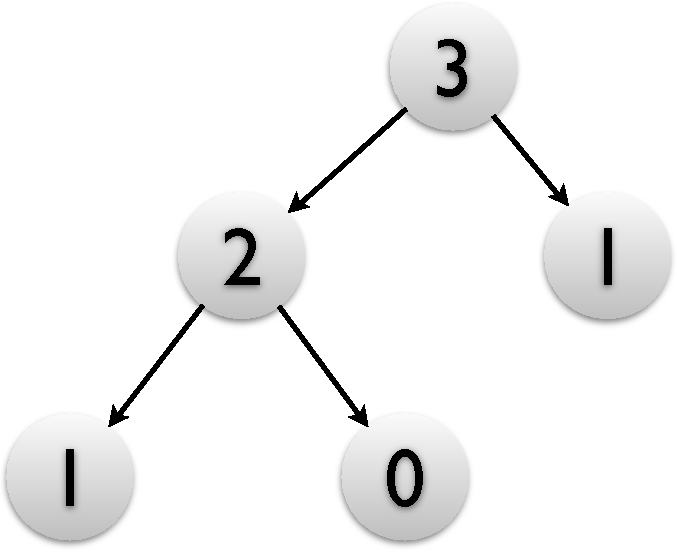
\includegraphics[width=\textwidth]{dag-dfg-crop}
      \end{center}
    \end{column}
  \end{columns}
\end{frame}
%------------------------------------------------------------------------------
\begin{frame}
  \frametitle{DAG of Fibonacci $n = 3$}
  \vspace{-10mm}
  \begin{center}
%    \hspace*{-6mm}
    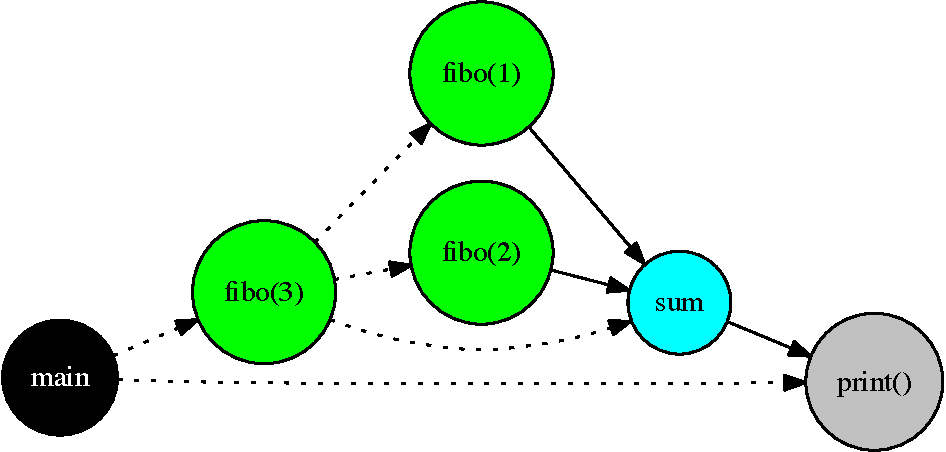
\includegraphics[width=\textwidth]{fibo/fibo4-clean-graph-crop}
  \end{center}
\end{frame}
%------------------------------------------------------------------------------
\begin{frame}
  \frametitle{DAG of Fibonacci $n = 3$}
  \vspace{-12mm}
  \begin{center}
    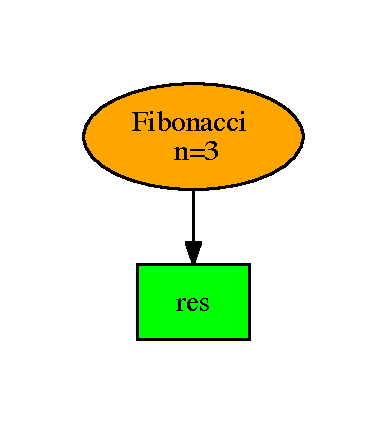
\includegraphics[scale=0.8]{fibo-graph-1}
  \end{center}
\end{frame}
%------------------------------------------------------------------------------
\begin{frame}
  \frametitle{DFG of Fibonacci $n = 3$}
  \vspace{-12mm}
  \begin{center}
    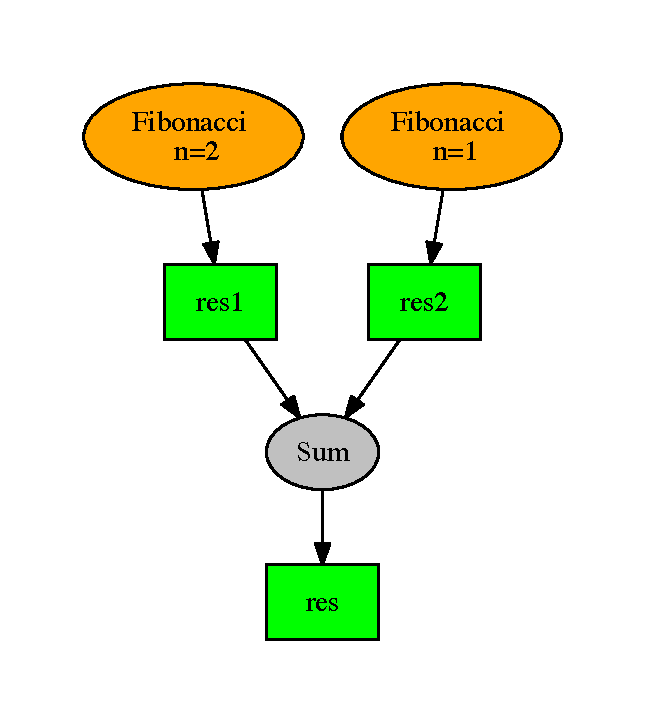
\includegraphics[scale=0.6]{fibo-graph-2}
  \end{center}
\end{frame}
%------------------------------------------------------------------------------
\begin{frame}
  \frametitle{DFG of Fibonacci $n = 3$}
  \vspace{-10mm}
  \begin{center}
    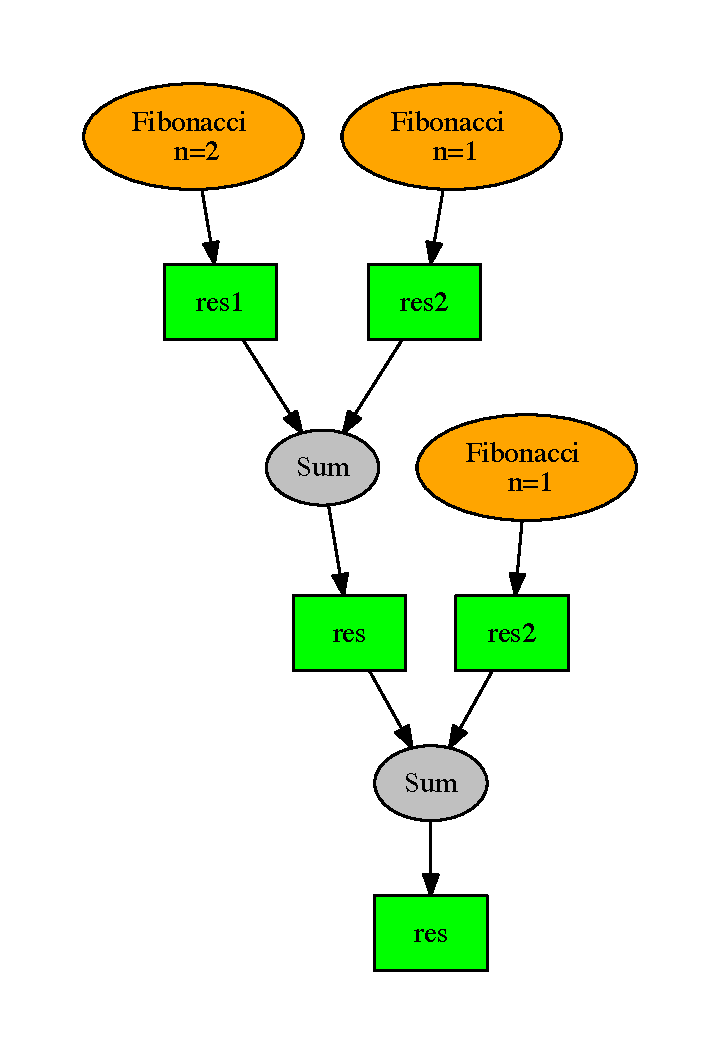
\includegraphics[scale=0.5]{fibo-graph-3}
  \end{center}
\end{frame}
%------------------------------------------------------------------------------
\begin{frame}
  \frametitle{DFG of Fibonacci $n = 3$}
  \vspace{-8mm}
  \begin{columns}
    \begin{column}{0.2\textwidth}
      \hspace*{-10mm}
      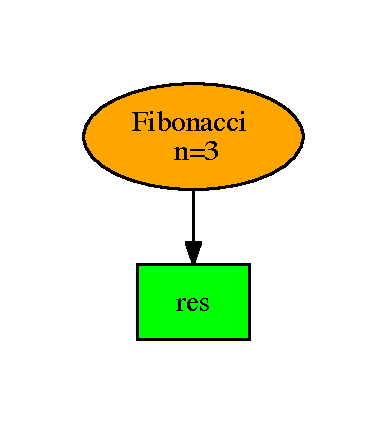
\includegraphics[scale=0.6]{fibo-graph-1}
    \end{column}
    %
    \begin{column}{0.4\textwidth}
      \hspace*{-10mm}
      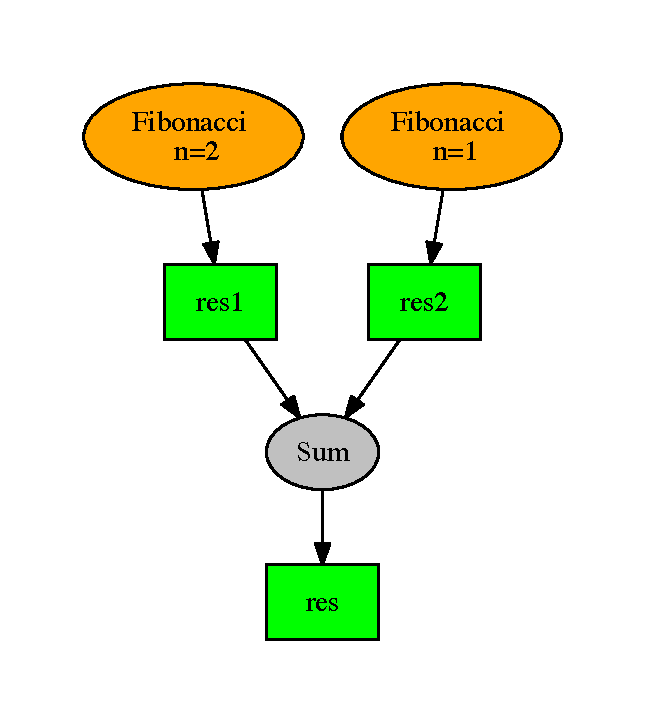
\includegraphics[scale=0.6]{fibo-graph-2}
    \end{column}
    %
    \begin{column}{0.4\textwidth}
      \hspace*{-10mm}
      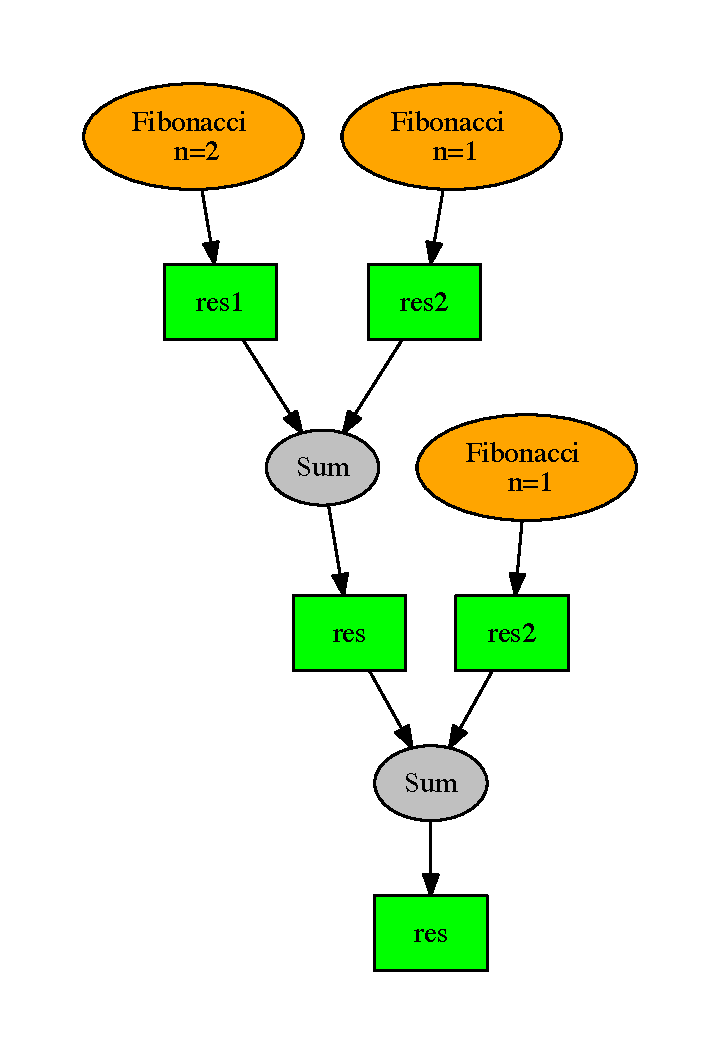
\includegraphics[scale=0.5]{fibo-graph-3}
    \end{column}
  \end{columns}
\end{frame}
%------------------------------------------------------------------------------
\begin{frame}
  \frametitle{DFG of Fibonacci $n = 3$}
  \vspace{-10mm}
  \begin{center}
%    \hspace*{-10mm}
    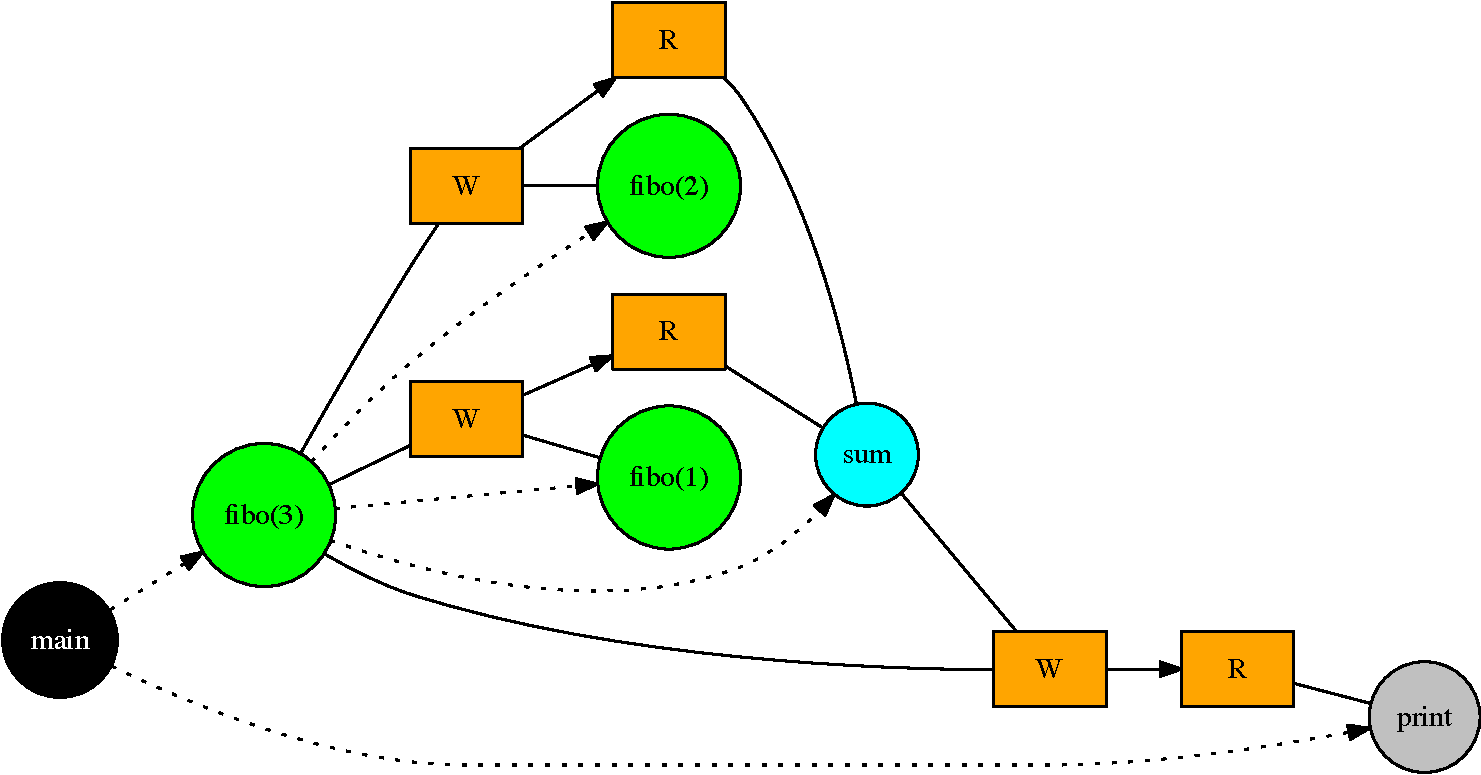
\includegraphics[width=\textwidth]{fibo/fibo4-graph-crop}
  \end{center}
\end{frame}
%------------------------------------------------------------------------------
\begin{frame}
  \frametitle{DFG of Fibonacci $n = 3$ (cumulative)}
  \vspace{-10mm}
  \begin{center}
%    \hspace*{-10mm}
    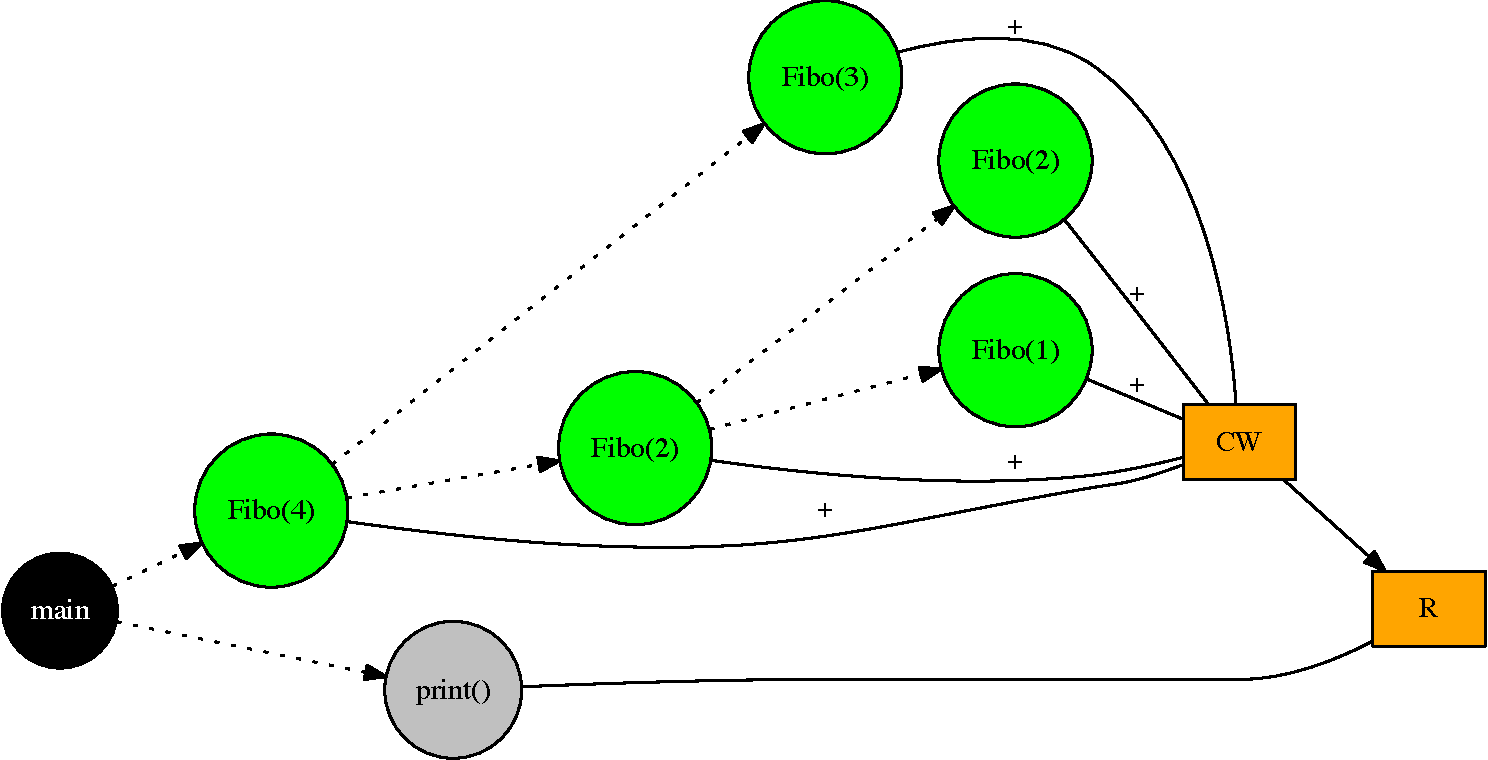
\includegraphics[width=\textwidth]{fibo/fibo4-cw-graph-crop}
  \end{center}
\end{frame}
%------------------------------------------------------------------------------
\begin{frame}
  \frametitle{DFG of Cholesky factorization}
  \vspace{-10mm}
  \begin{center}
%    \hspace*{-10mm}
    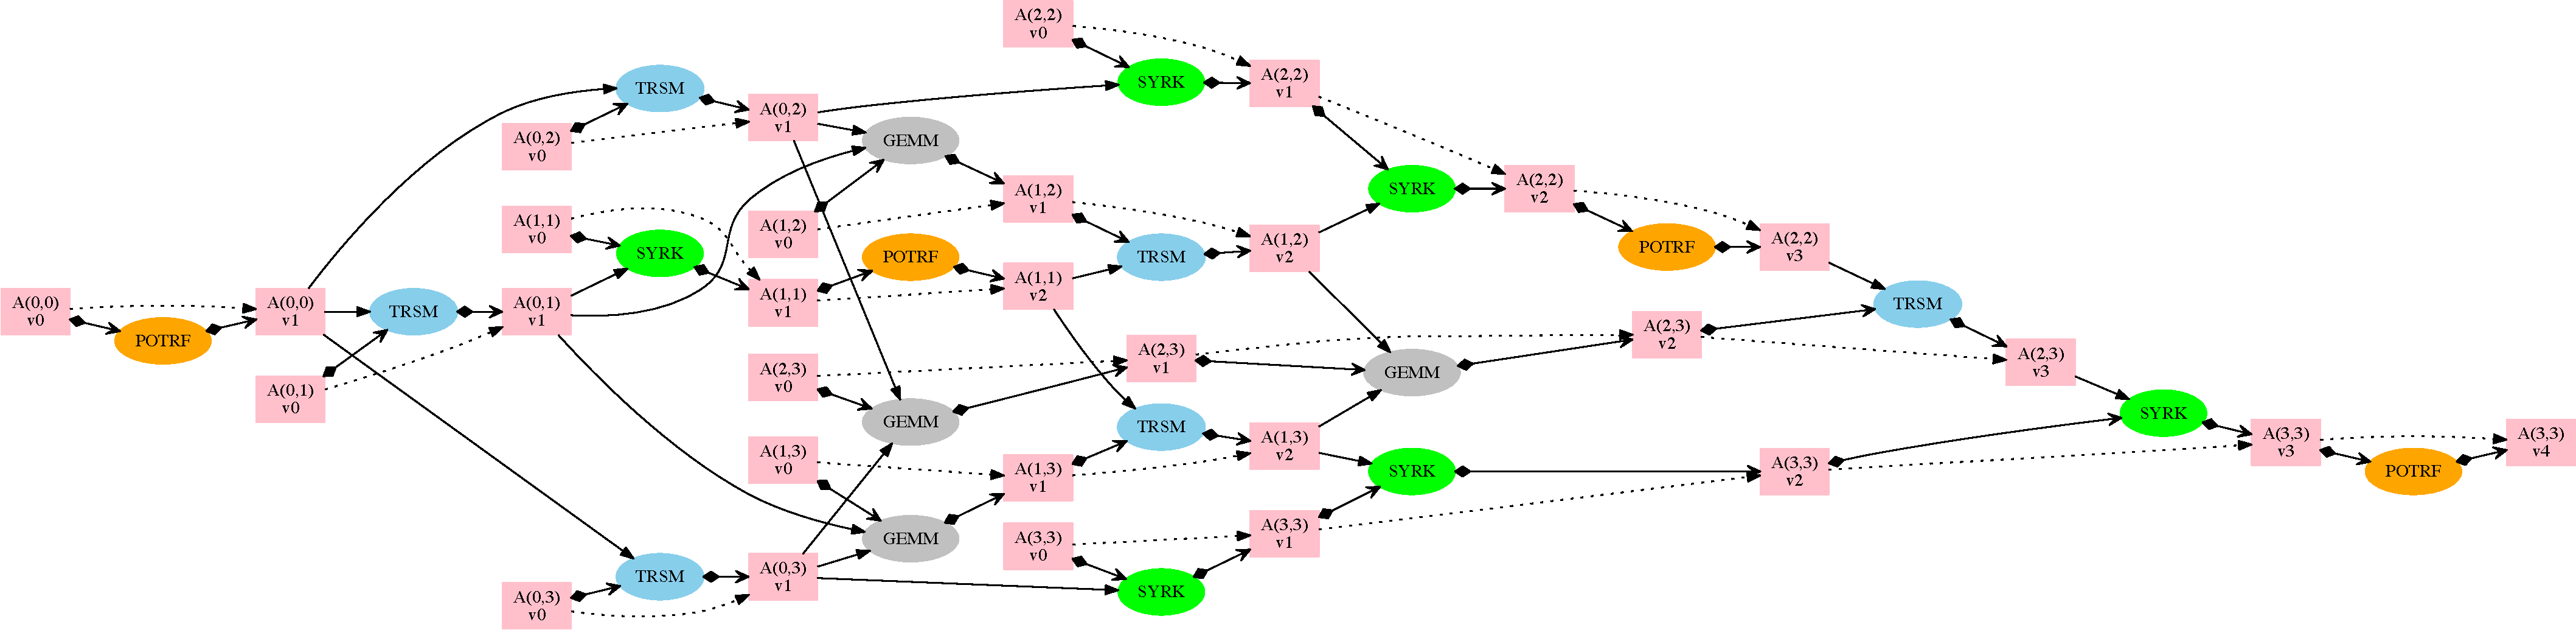
\includegraphics[width=\textwidth]{graph-cholesky-DFG-crop}
  \end{center}
\end{frame}
%------------------------------------------------------------------------------
\begin{frame}
  \frametitle{DFG of Cholesky factorization}
  \vspace{-2mm}
  \begin{center}
    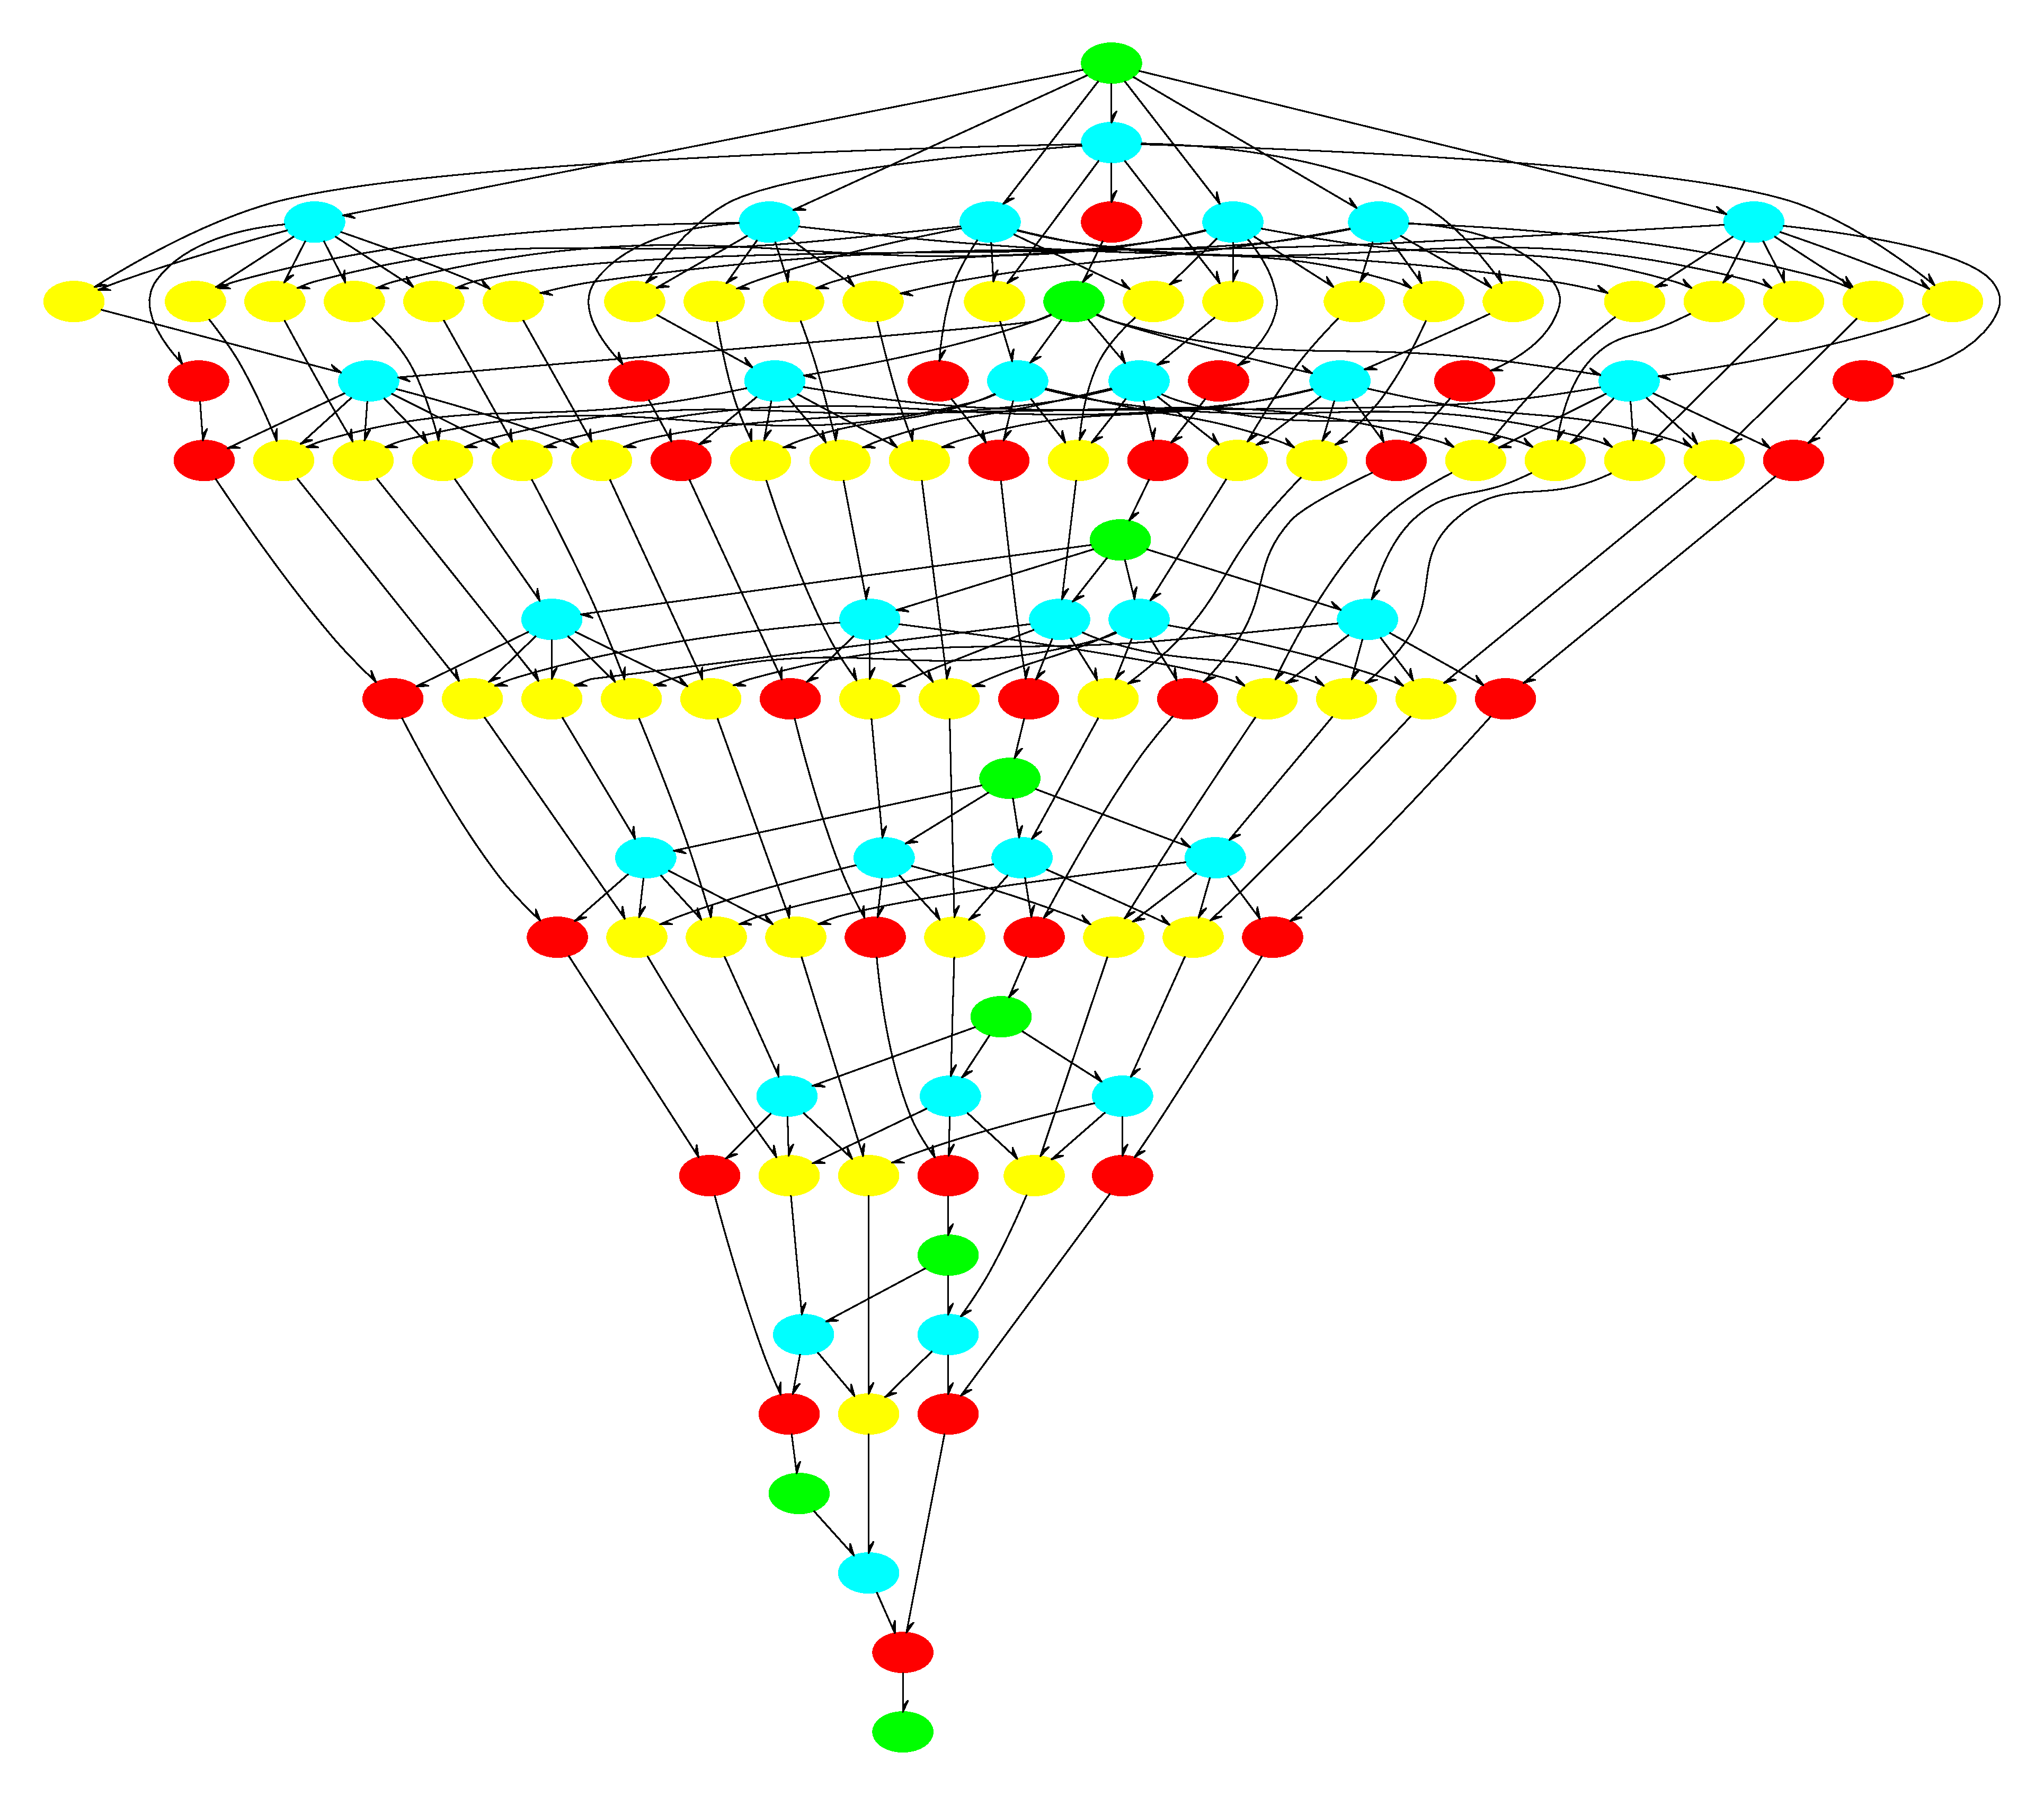
\includegraphics[width=0.8\textwidth]{cholesky}
  \end{center}
\end{frame}
%------------------------------------------------------------------------------
\begin{frame}
  \frametitle{DFG of Blocked matrix multiplication}
  \vspace{-10mm}
  \begin{center}
%    \hspace*{-10mm}
    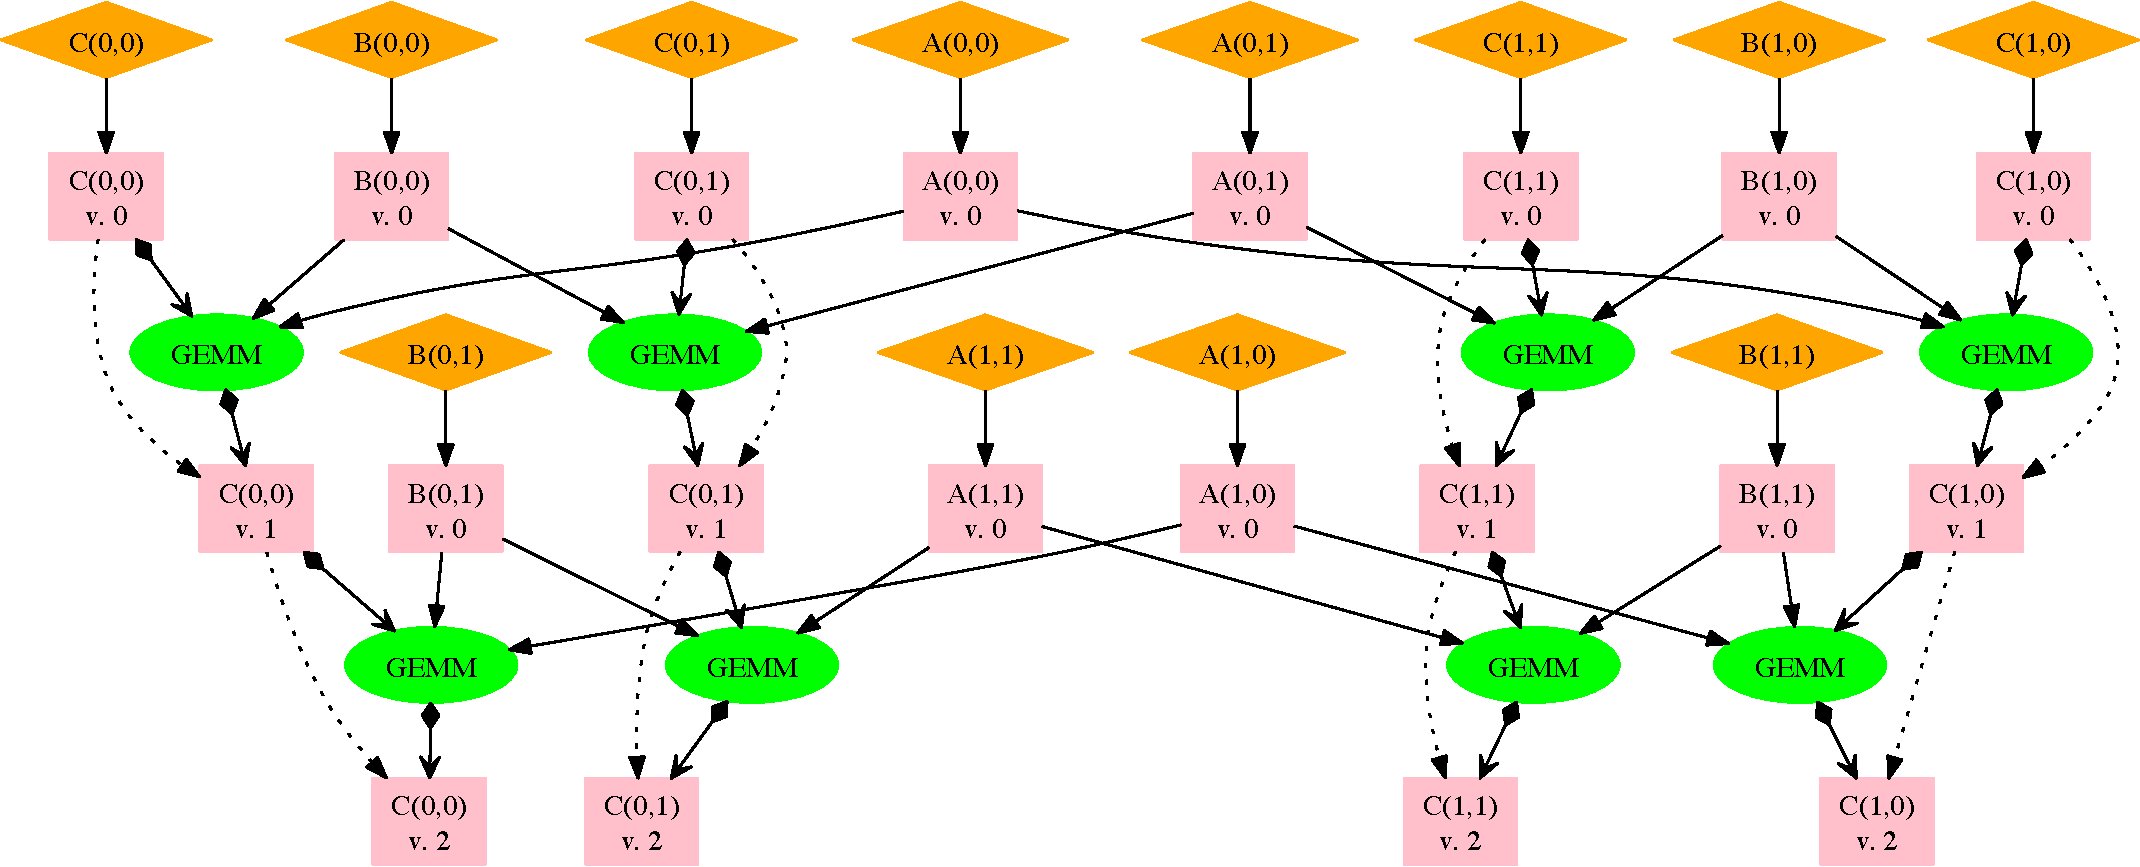
\includegraphics[width=\textwidth]{graph-gemm-DFG-crop}
  \end{center}
\end{frame}
%------------------------------------------------------------------------------
